\documentclass[]{cv-style} % Add 'print' in [] to get print-view
\usepackage{graphicx}
\usepackage[utf8]{inputenc}
\usepackage{url}
\usepackage{hyperref}

% \inputencoding{utf8}
% \usepackage{unixode}

\hypersetup{
    colorlinks,
    citecolor=black,
    filecolor=black,
    linkcolor=black,
    urlcolor=black
}

\newcommand{\heart}{\ensuremath\varheartsuit}

%%%%%%%%%%%%%%%%%%%%%%%%%%%%%%%%%%%%%%%%%%%%%%%%%%%%%%%%%%%%%%%%%%%%%%%%%%%%%%%%
\begin{document}
\header{Matteo}{DeCarlo}

%%%%%%%%%%%%%%%%%%%%%%%%%%%%%%%%%%%%%%%%%%%%%%%%%%%%%%%%%%%%%%%%%%%%%%%%%%%%%%%%
%%%%%%%%%%%%%%%%%%%%%%%%%%%%%%%%%%%%%%%%%%%%%%%%%%%%%%%%%%%%%%%%%%%%%%%%%%%%%%%%
\begin{aside}
%\section{ }
~
~
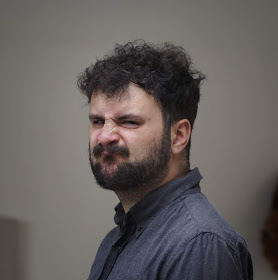
\includegraphics[width=5cm]{2018}
\section{Contact}
Panamakade 27
Amsterdam - 1019AX
Netherlands
~
+31 6 15653505
~
matteo.dek@gmail.com
matteo.dek@covolunablu.org
\section{Languages}
Italian mother tongue
English fluency
\section{Skills}
Programming
AI/Machine Learning
Continuous Integration
OS (Linux, Windows, Mac)
Docker
\section{Programming Laguages}
C
\heart \hspace{1pt} C++
\heart \hspace{1pt} Rust
Python
Java
Javascript
\section{Frameworks}
Qt
Opengl
Vulkan
AngularJS
\end{aside}

%%%%%%%%%%%%%%%%%%%%%%%%%%%%%%%%%%%%%%%%%%%%%%%%%%%%%%%%%%%%%%%%%%%%%%%%%%%%%%%%
%%%%%%%%%%%%%%%%%%%%%%%%%%%%%%%%%%%%%%%%%%%%%%%%%%%%%%%%%%%%%%%%%%%%%%%%%%%%%%%%
\section{Career Objective}
  \vspace{-0.2cm}
Looking for a career in the interactive storytelling industry, where immersive stories and challenging gameplays are created. Hopeful to find an environment where I can learn about graphic programming as done in the industry and to apply and improve my artificial intelligence skills. Also very passionate about space exploration, rocket science and photography.

%%%%%%%%%%%%%%%%%%%%%%%%%%%%%%%%%%%%%%%%%%%%%%%%%%%%%%%%%%%%%%%%%%%%%%%%%%%%%%%%
\section{Experience}
\begin{entrylist}
\entry
  {2014 - Now}
  {Stormbits}
  {Amsterdam, Netherlands}
  {\jobtitle{Junior Software Engineer}\\
Complete rewrite of a web application. Only maintainer of the frontend for web applications (AngularJS). Responsible for design and UX choices. Android Apps prototyping. Simple, single page web applications rapid design and development.}
\entry
  {2015}
  {Vrije Universiteit}
  {Amsterdam, Netherlands}
  {\jobtitle{Research Assistant}\\
Modular robot controller development based on \textbf{C}entral \textbf{P}attern \textbf{G}enerators (C++). Code organization and cleanup. Creation of debug and analysis tools.\\}
\end{entrylist}

%%%%%%%%%%%%%%%%%%%%%%%%%%%%%%%%%%%%%%%%%%%%%%%%%%%%%%%%%%%%%%%%%%%%%%%%%%%%%%%%
\section{Education}
\begin{entrylist}
\entry
{2014 - 2018}
{Master {\normalfont in Computer Science [waiting]}}
{Amsterdam, Netherlands}
{Average: 7.9 out of 10\newline
Branch: \jobtitle{Technical Artificial Intelligence}\newline
Thesis: Evolving SUPG-based closed loop controllers for modular robots of arbitrary shapes\newline
Vrije Universisteit - Netherlands}
\entry
{2009 - 2014}
{Bachelor {\normalfont in Computer Science [104 out of 110]}}
{Modena, Italy}
{Thesis: Random generation of people trajectories for virtual smart floors\newline
Università di Modena e Reggio Emilia}
\end{entrylist}

%%%%%%%%%%%%%%%%%%%%%%%%%%%%%%%%%%%%%%%%%%%%%%%%%%%%%%%%%%%%%%%%%%%%%%%%%%%%%%%%
\section{Publications}
\begin{entrylist}
\entry
{2017}
{Real-World Evolution of Robot Morphologies: A Proof of Concept}
{VU}
{Article}
\entry
{2016}
{Improving RL Power for On-Line Evolution of Gaits in Modular Robots}
{VU}
{Conference Paper}
\end{entrylist}

%%%%%%%%%%%%%%%%%%%%%%%%%%%%%%%%%%%%%%%%%%%%%%%%%%%%%%%%%%%%%%%%%%%%%%%%%%%%%%%%
\section{Example Projects}
\begin{entrylist}
\entry
{}
{Mars Rotating Live Wallpaper}
{Android}
{\href{https://git.covolunablu.org/portaloffreedom/MarsWallpaper}{Source Code}}
\entry
{2008 - 2009}
{APAC}
{AIUB}
{Worked with the Organizer Team}
\end{entrylist}

%%%%%%%%%%%%%%%%%%%%%%%%%%%%%%%%%%%%%%%%%%%%%%%%%%%%%%%%%%%%%%%%%%%%%%%%%%%%%%%%
\section{Reference}
\begin{entrylist}
\entry
{Senior Manager}
{Md. Shariful Islam}
{Summit Communications Limited}
{md.shariful@summitcommunications.net}
\end{entrylist}
\end{document}